% IEEE Paper Template for US-LETTER Page Size (V1)
% Sample Conference Paper using IEEE LaTeX style file for US-LETTER pagesize.
% Copyright (C) 2006-2008 Causal Productions Pty Ltd.
% Permission is granted to distribute and revise this file provided that
% this header remains intact.
%
% REVISION HISTORY
% 20080211 changed some space characters in the title-author block
%
\documentclass[10pt,conference,letterpaper]{IEEEtran}
\usepackage{times,amsmath,epsfig}
%
\title{A Light-weight API for Multicore Programming}
%
\author{
Author: TBA
%{Christopher G. Baker {\small $~^{\#1}$}, H. Carter Edwards {\small $~^{*2}$}, Michael A. Heroux {\small $~^{\#3}$}, Alan B. Williams {\small $~^{*4}$} }%
%% add some space between author names and affils
%\vspace{1.6mm}\\
%\fontsize{10}{10}\selectfont\itshape
%% 20080211 CAUSAL PRODUCTIONS
%% separate superscript on following line from affiliation using narrow space
%$^{\#}$\,Scalable Algorithms Department, Sandia National Laboratories\\
%P.O. Box 5800, MS 1320, Albuquerque, NM 87185-1320, USA\\
%\fontsize{9}{9}\selectfont\ttfamily\upshape
%$^{1}$\,cgbaker@sandia.gov\\
%$^{3}$\,maherou@sandia.gov%
%% add some space between email and affil
%\vspace{1.2mm}\\
%\fontsize{10}{10}\selectfont\rmfamily\itshape
%$^{*}$\,Computational Simulation Infrastructure Department, Sandia National Laboratories \\
%P.O. Box 5800, MS 0382, Albuquerque, NM 87185-0382, USA\\
%\fontsize{9}{9}\selectfont\ttfamily\upshape
%$^{2}$\,hcedwar@sandia.gov\\
%$^{4}$\,william@sandia.gov%
}
%
\begin{document}
\maketitle
%
\begin{abstract} 
Multicore nodes have become ubiquitous in just a few years.  At the same time, writing portable parallel software for multicore nodes is extremely challenging.  Widely available programming models such as OpenMP and Pthreads are not useful for devices such as graphics cards, and more flexible programming models such as RapidMind are only available commercially.  OpenCL represents the first truly portable standard, but its availability is limited.  In the presence of such transition, we have developed a minimal application programming interface (API) for multicore nodes that allows us to write portable parallel linear algebra software that can use any of the aforementioned programming models and any future standard models. We utilize C++ template meta-programming to enable users to write parallel kernels that can be executed on a variety of node types, including Cell, GPUs and multicore CPUs. The support for a parallel node is provided by implementing a Node object, according to the requirements specified by the API. This ability to provide custom support for particular node types gives developers a level of control not allowed by the current slate of proprietary parallel programming APIs. We demonstrate implementations of the API for a simple vector dot-product on sequential CPU, multicore CPU and GPU nodes.
\end{abstract}

% NOTE keywords are not used for conference papers so do not populate them
% \begin{keywords}
% keyword-1, keyword-2, keyword-3
% \end{keywords}
%
\section{Introduction}
%

Multicore and manycore processors have become the standard building block for desktop and scalable computers. The relationship between clock rate and power consumption, coupled with a limited ability to handle dissipated heat, means that performance improvements are now coming in the form of a growing number of parallel cores instead of an increased clock rate. While multicore processors have been present in distributed-memory systems since the early 1990s, the majority of scientific applications for these system were developed using only a distributed memory model. This is not to suggest that multiple cores per node have not been useful; scientific codes using a distributed-memory programming model (e.g., MPI) can benefit from multicore nodes treating each core as a node unto itself. In the particular case of a distributed-memory code using MPI, a cluster of $m$ nodes with $k$ cores per node can be launched with $p=m*k$ MPI processes. This MPI-only approach is popular, due to its simplicity and current success~\cite{HerouxThoughts}. However, it is unlikely that this approach will continue to scale as we move from moderately multicore nodes (approx. 10 cores per node) to manycore nodes (tens or hundreds of cores per node). Even now it is clear that some important primitives can benefit from an explicitly shared-memory programming approach. Furthermore, if hardware requirements continue to favor increasing levels of parallelism over increasing clock frequencies, sequential codes will no longer see the gradual improvement that was experienced in the past. It will then be necessary to exploit some level of parallelism to see continued speed-up on future processors. 

Another disadvantage of the distributed-memory approaches is that they are typically aimed at programming general purpose processors and are less amenable to the current generation of special-purpose multicore and manycore processors (e.g., GPU, STI Cell, FPGA). These special-purpose processors constitute another reason for the recent attention on multicore computing. Their rapidly increasing power and programmability motivates their appeal for scientific computing. Modern desktops and workstations include graphics processing units (GPUs) with hundreds of programmable cores, whose combined computational power often eclipses the system's CPU. The hardware support for parallelism, as well as the superior memory bandwidth on these devices, has made them a target for high-performance computing. At the same time, the introduction of numerous APIs for programming GPUs for general-purpose computing has removed the need to employ graphics-specific languages. For example, NVIDIA has developed the CUDA~\cite{CUDA} architecture for programming recent GPUs from the company, and similar efforts are underway to support architectures from other hardware vendors~\cite{AMDStream,BrookGPU}. The use of special-purpose hardware is not limited to GPUs. The Los Alamos Roadrunner~\cite{Roadrunner} utilizes STI Cell processors similar to those used in the Sony Playstation~3 video game console, whereas the Anton supercomputer~\cite{Anton} uses custom-built hardware for the solution of a specific scientific problem (molecular dynamics). In the case of the Roadrunner supercomputer, it is necessary to harness the Cell co-processors as they constitute most of the computational power of the computer.

The diversity of multicore hardware platforms has motivated the creation of a number of approaches for programming them. As previously mentioned, one popular approach for handling homogenous multicore nodes is to apply current distributed-memory programming models to the individual cores. Alternatively, there are a number of shared-memory programming models, with Pthreads and OpenMP being the most popular; a more recent effort is Intel's Thread Build Blocks (TBB)~\cite{TBB}. For heterogenous multicore nodes, there are at least as many programming models as there are architectures. Recently there have been several attempts to define a programming environment that can be targeted to diverse architectures, including multicore CPUs, GPUs and the STI Cell. RapidMind's proprietary Multicore Development Platform~\cite{RapidMind} provides a single C++ programming interface capable exploiting multiple back-ends. More recently, the OpenCL~\cite{OpenCL} effort has defined an open standard for programming multicore processors. With backing from numerous hardware and software vendors, this framework consists of a new language (based on C) for writing parallel kernels.

In this paper, we propose a minimal, light-weight API for writing kernels for parallel execution on multicore compute nodes. We can develop such an API because, even though there are many competing multicore and manycore programming models, there is a common work-data registration and execution model that works across all of them.  Similar to TBB and RapidMind, our API exploits C++ template metaprogramming to enable user kernels to be compiled to a generic threaded back-end. Like OpenCL and RapidMind, these kernels can be compiled to a diversity of parallel architectures. Unlike the aforementioned, the proposed API is fully open. Our motivation is not in developing new APIs to compete with current standards. However, the current solutions are not sufficiently portable, as they address a limited number of computing scenarios. More significantly, the current solutions focus mainly on the manner in which parallel kernels are written, leaving little (if any) ability to specify the manner in which those kernels are executed. The proposed API allows application developers to write parallel kernels, while also allowing node developers full flexibility in support mission-critical node types.

\section{Programming Model and Interface}

% API will expand to support other concepts: mutex, atomics, other parallel operations

The concept at the center of the proposed node-programming API is that of a \emph{compute node}. The API defines the node as a C++ class that implements a specified interface, defining necessary types and implementing required methods. To perform a parallel computation, a user defines the work and data constituting the computation. These items are encapsulated into a \verb!struct!; the data members are variable, depending on the nature of the computation, while the work is contained in API-defined struct member functions dictated according to the type of parallel computation (e.g., parallel \verb!for!, parallel reduce). 

\begin{figure}[h]
	\centerline{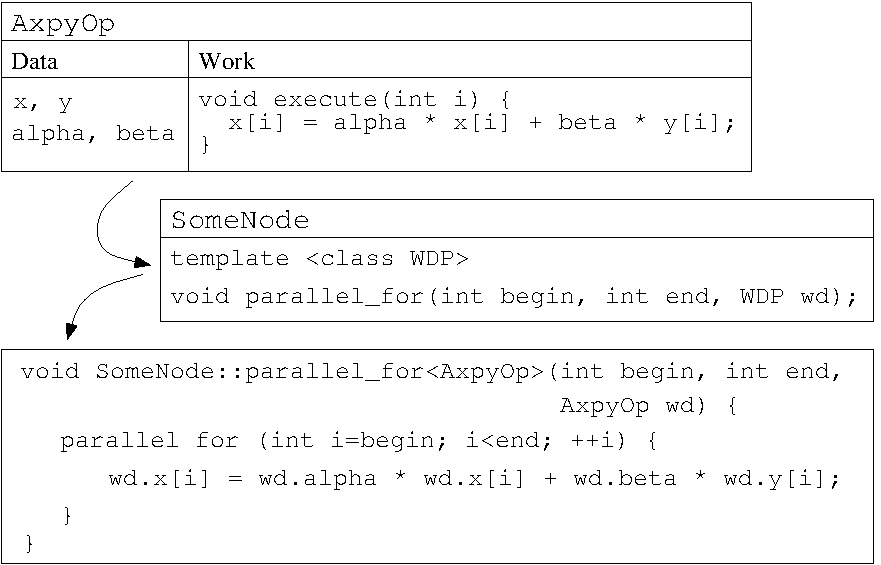
\includegraphics[width=8.5cm]{AxpyExample.pdf} }
	\caption{Example of a vector Axpy operation under the proposed API.}
	\label{fig:axpy}
\end{figure}

Figure~\ref{fig:axpy} illustrates this arrangement for a simple vector axpy operation implemented via a parallel \verb!for! loop. The data members of the \verb!AxpyOp! struct are set by the caller at runtime; the quantity and type of these members are particular to the axpy operation. The \verb!AxpyOp! object is passed to the \verb!parallel_for! computational method of the chosen node object; each compute node is required to implement this method. This method is templated on a work-data pair struct, and it is required that the struct (\verb!AxpyOp!, in this case) implement a method \verb!execute()!. At compile time, a parallel \verb!for! loop, as implemented by the particular node, is instantiated using the \verb!execute()! operation, resulting in a parallel axpy operation. By using this same struct with a different node implementation, the code defining the parallel kernel (in this case, the \verb!execute()! routine) can be compiled multiple times for multiple compute node implementations, capturing the ``write once, run anywhere'' capability of OpenCL and RapidMind.

The proposed API there consists of two parts: the requirements placed on node objects, and the requirements placed on the user kernels that are submitted to node objects. The structure of the node objects can be divided into two parts: the memory model and the parallel computational routines. The memory model defines the concept of a \emph{compute buffer} and the routines for interacting with these buffers. A compute buffer is a region of memory available for computation via parallel kernels. These memory objects are not available for use directly by non-kernel code, nor are parallel kernels able to access any memory resources aside from compute buffers. In the particular case of the axpy example in Figure~\ref{fig:axpy}, the arrays \verb!x! and \verb!y! are compute buffers, and the node implementation specifies everything about them: where and how they are allocated and deallocated, how they are indexed, and how they are accessed by non-kernel code. The second purpose of the API is to specify the parallel computational routines provided by a compute node, as well as the requirements on a work-data pair necessary for each parallel computational routine.

\subsection{Memory Model} 

The compute buffer is not a fixed type under the API, but instead is specified individually by each node implementation. Given a node type \texttt{Node}, a user declares a compute buffer of type \verb!float! like so:
{\small \begin{verbatim}
Node::buffer<float>::buffer_t my_buff;
\end{verbatim}}
This code simply declares a buffer object \verb!my_buff!, which references a float-valued region of memory intended for use in a parallel kernel. The decision to use node-specific arrays was intended to enable maximum flexibility and efficiency on nodes with unique memory architectures. In particular, we were concerned with compute nodes matching a host-device model, where the host main memory is distinct from that of the device where the parallel computations will occur. However, for many node implementations, \verb!buffer<T>::buffer_t! will simply map to the pointer type \verb!T *!. The only requirement on the buffer type is that it supports the standard C array indexing via the bracket operator, like \verb!my_buff[i]!. This is of course automatic for buffers implemented simply as a C pointer; for any other type, the buffer will need to overload the \verb!operator[]! method. Furthermore, the API requires only that this functionality be supported for kernel code executed via one of the parallel computation routines. In the general case, the indexing of compute buffers in non-kernel code yields undefined results. Future requirements may include assignment of buffers and pointer-arithmetic. 

The compute buffer \verb!my_buff! declared above must be allocated before it can be used. This is done via the node's buffer allocation method:
{\small \begin{verbatim}
template <class T>
Node::buffer<T>::buffer_t
Node::allocBuffer(int length); 
\end{verbatim}}
\noindent Before allocation, use of a compute buffer is undefined. Accepting a single argument \verb!length!, this method allocates a compute buffer of sufficient size to store \verb!length! number of values of type \verb!T!. Even for mundane implementations of the buffer type, the requirement to allocate compute buffers using the \verb!allocBuffer()! method might allow particular node implementations to improve performance (e.g., via more efficient memory layout on NUMA architectures). When an allocated buffer is no longer needed, it should be deallocated using the \verb!freeBuffer()! method:
{\small \begin{verbatim}
template <class T>
void Node::freeBuffer(
   Node::buffer<T>::buffer_t buff
);
\end{verbatim}}
\noindent After calling \verb!freeBuffer()!, use of a compute buffer is undefined.

Of course, the application developer needs to be able to write to a compute buffer to prepare for computation, and likewise needs the ability to read from a compute buffer to determine the results of said computation. The proposed API defines six methods to address varying use cases. Three of these methods employ copy semantics, to duplicate the results of data from one location (compute buffer or main memory) to another. The other three methods employ view semantics, giving effectively direct access to the contents of a compute buffer. The latter are not strictly necessary for the purpose of initializing and evaluating parallel computation, but they can in many cases be more efficient than using copy semantics.

{\small \begin{verbatim}
template <class T>
void Node::copyToBuffer( int size, 
  const T * src,
  Node::buffer<T>::buffer_t dest, 
  int dest_offset
);                    

template <class T>
void Node::copyFromBuffer( int size, 
  Node::buffer<const T>::buffer_t src, 
  int src_offset, 
  T * dest
);                    

template <class T>
void Node::copyBuffers( int size, 
  Node::buffer<const T>::buffer_t src, 
  int src_offset, 
  Node::buffer<T>::buffer_t dest, 
  int dest_offset );                    
\end{verbatim}}
\verb!copyToBuffer()! copies data in main memory to the specified compute buffer, so that \verb!dest[dest_offset+i]! is equal to \verb!src[i]! for \verb!i=0,...,size-1!. The call may be implemented in an asynchronous manner. However, the API guarantees that upon return, it is safe to write to the memory at \verb!src!, and that the effect of the copy will be complete before the buffer \verb!dest! is used by the compute node. Similarly, \verb!copyFromBuffer()! copies data from a compute buffer to the main memory. This method is guaranteed to return only after the memory transfer is complete. The method \verb!copyBuffers()! copies data from one compute buffer to another. This method may be asynchronous, but as with \verb!copyToBuffer()!, the effect is guaranteed to be complete before either buffer is needed by a parallel computation or another memory operation.

{\small \begin{verbatim}
template <class T>
T * Node::viewBuffer(
  bool writeOnly, int size, 
  Node::buffer<T>::buffer_t buff, 
  int offset
);
  
template <class T>
const T * Node::viewBufferConst(
  int size,
  Node::buffer<const T>::buffer_t buff,
  int offset
);
  
template <class T>
void Node::releaseView(
  Node::buffer<T>::buffer_t buff
);
\end{verbatim}}
The \verb!viewBuffer()! method returns a pointer to a location in main memory containing the contents of the specified compute buffer. This method is intended to allow more efficient access for writing to the parallel buffer than may possible via the copy methods. The write-only flag specifies that the view will be written to but not read from; in this case, the data in the view is undefined. If the data must be read and written to, this flag should be set to false. Any changes made to the buffer via its view are not required to take effect in the buffer until the view is released (see \verb!releaseView()!). If the buffer view is read-only, the user is encouraged to create the view using \verb!viewBufferConst()!. This method is intended to allow more efficient read-only access to a compute buffer. For both \verb!viewBuffer()! and \verb!viewBufferConst()!, the created view should be passed to \verb!releaseView()! so that any allocated resources can be recovered.

{\small \begin{verbatim}
void Node::readyBuffers(
  Node::buffer<const void>::buffer_t cbuffs[],  
  int numConstBuffers,
  Node::buffer<void>::buffer_t ncbuffs[], 
  int numNonConstBuffers
);
\end{verbatim}}
The final memory routine is \verb!readyBuffers()!. This routine accepts two arrays, one to a list of const-valued compute buffers, one to a list of non-const-valued compute buffers. Before using any compute buffer in a parallel routine, it is required that the buffers be ``readied'' by this routine. The purpose of this routine is to ensure that the necessary compute buffers are optimally prepared for parallel computation.

\subsection{Parallel Computing Model}

The memory model specified by the API and the implementation of that model for a particular node are critical for achieving good performance. However, the heart of the API is in the parallel computational routines that execute user kernels. Currently, the API describes only two parallel structures: the parallel \verb!for! loop and the parallel reduction. Future releases of the API will add more parallel routines, as well as fine-grained parallel utilities such as atomics.

{\small \begin{verbatim}
template <class WDP>
void Node::parallel_for(
   int beg, int end, WDP wd
); 

struct WDP {
  void KERNEL_PREFIX execute(int i);
};
\end{verbatim}}
This \verb!parallel_for! method, as suggested by its name, implements a \verb!for! loop in parallel, where the \verb!execute()! method of the prescribed work-data pair provides the body of the \verb!for! loop. The underlying assumption of a parallel \verb!for!  is that there is no dependence between the loop iterations, allowing them to be executed simultaneously and in any order. The semantics of the \verb!parallel_for! method dictate that \verb!wd.execute(i)! will be called exactly once for each index \verb!i! in \verb![beg,end)!. The \verb!KERNEL_PREFIX! occurrence is a macro that can be expanded to provide additional compiler pragmas when necessary/useful for particular platforms (e.g., CUDA's \verb!__device__! pragma).

{\small \begin{verbatim}
template <class WDP>
typename WDP::ReductionType
Node::parallel_reduce(
   int begin, int end, WDP wd
); 

struct WDP {
  typedef  ...  ReductionType;

  KERNEL_PREFIX ReductionType identity();
  KERNEL_PREFIX ReductionType generate(int i);
  KERNEL_PREFIX ReductionType 
     reduce(ReductionType x, ReductionType y);
};
\end{verbatim}}
A reduction operation is a computation that combines a set of values via some associative \emph{reduction operator} (e.g., sum, product, min, max). A parallel reduction performs this operation in parallel, typically by performing a parallel fan-in, under the assumption that the entries can be generated and reduced in any order. The API requires that to be used with \verb!parallel_reduce()!, a work-data pair struct must define a typedef \verb!ReductionType!, indicating the value type for the reduction operation, as well as the following methods:
\begin{itemize}
\item a method \verb!generate()!, which generates the values to be reduced;
\item  a method \verb!reduce()!, which accepts two \verb!ReductionType! arguments and performs the reduction operator; and
\item a method \verb!identity()!, which specifies a \verb!ReductionType! element representing the identity under the operation \verb!reduce()!.
\end{itemize}The implementation of \verb!parallel_reduce()! will return the reduction of all generated values in the range \verb![begin,end)!, having called \verb!generate()! exactly once for each of the indices in that range (the latter is useful, as it permits predictable behavior in scenarios where the \verb!generate()! method has side-effects.)

\section{Example Nodes}

The following sections describe two different implementations of the proposed node API, for the purpose of illustrating the individual components. These nodes effectively wrap the Intel TBB and NVIDIA CUDA parallel interfaces.

\subsection{Intel TBB}

This section discusses the implementation of a node class \verb!TBBNode! corresponding to a Intel Threading Building Blocks~(TBB) back-end. Intel TBB~\cite{TBB} is a C++ library using templates which allows users to write code to be run on a homogenous multicore CPU. The benefit of TBB is that it frees the user from concern regarding the complications of the thread library for the particular system; threads are initialized once by the TBB runtime, then assigned to parallel tasks whenever the user passes work to TBB.

Because there is no distinction between the main memory and the memory used for parallel computation, the memory model for \verb!TBBNode! is straight-forward. The buffer type is a simple C pointer; i.e., \verb!TBBNode::buffer<T>::buffer_t! is simply \verb!T *!. The buffer allocation and deallocation can be implemented, for example, via the \verb!malloc()! and \verb!free()! standard C routines. The buffer copy methods are implemented via some standard copy method (e.g., \verb!memcpy()! or \verb!std::copy()!); the view creation method simply returns the appropriate pointer into the buffer, and \verb!releaseView()! is a no-op.

All that remains for \verb!TBBNode! is to implement the \verb!parallel_for()! and \verb!parallel_reduction()! methods. The TBB library provides similar functionality via the \verb!tbb::parallel_for()! and \verb!tbb::parallel_reduce()! methods. As with the proposed API, these methods exploit C++ templates and compile-time polymorphism to enable the user to specify both the work and the data defining these operations. In implementing the \verb!TBBNode! class to target this back-end, it is simply a matter of wrapping our work-data pairs into the form expected by TBB and passing these on to the parallel \verb!for! and parallel reduction methods of TBB. Because both the proposed API and TBB have explicitly defined interfaces, it is trivial to write adaptors from the former to the latter.

\subsection{NVIDIA CUDA}

The effort in implementing a node for a GPU is significantly harder than for the TBB case. To begin with, the TBB library provided implementations for the required parallel computations, whereas CUDA will require some amount of development specific to GPU platform. This development will necessarily be conducted in the CUDA language (as opposed to C/C++), and ultimately the relevant code must be passed through the CUDA compiler. Furthermore, due to the host-device divide currently present for most GPU platforms, the effort in implementing the memory model for this node will certainly exceed that required, for example, by the TBB node. Our current proof-of-concept implementation of a CUDA compute node allocates both host and device memory for each compute buffer. By keeping track of dirty bits, this enables the node implementation to be very frugal regarding expensive data movements between host and device memory.

Regarding the implementation of the parallel computation routines, the CUDA framework makes implementing \verb!parallel_for()! rather easy. The parallel reduction algorithm is a little more complicated, but numerous resources~\cite{CUDA} outline methods for performing this operation with maximal efficiency. The only change to these is to ensure that the \verb!generate()! and \verb!reduce()! methods of the work-data pair object are used appropriately.

\subsection{Numerical Results}

For testing purpose, we implemented the proposed API for three node types: a trivial sequential node called \verb!SerialNode!; a interface to Intel TBB called \verb!TBBNode!; and a node using CUDA for NVIDIA GPUs called \verb!CUDANode!. These nodes were evaluated using a simple inner product, computed using the node's \verb!parallel_reduce()! functionality coupled with the following dot-product kernel:
{\small \begin{verbatim}
template <class Node>
struct DotOp {
  typename Node::template 
     buffer<const float>::buffer_t  x, y;
     
  typedef  float  ReductionType;
  
  static KERNEL_PREFIX float
    identity()                { return 0.0f; }
  KERNEL_PREFIX float 
    generate(int i)      { return x[i]*y[i]; }
  KERNEL_PREFIX float
    reduce(float x, float y)   { return x+y; }
};
\end{verbatim}}

The results for the three node implementations, for varying problem sizes, are shown in Table~\ref{tbl:results}. The SerialNode yields consistent performance for the tested vector lengths, while larger vector lengths better amortize the latency involved in launching the multi-threaded kernels associated with the TBB and CUDA implementations. For the largest tested problem size, the TBB and CUDA implementation provide 3.5x and 6x speedup, respectively, over the serial implementation.

\begin{table}[!h]
\centering

\caption{Dot-product results for SerialNode, TBBNode, and CUDANode implementations. 
CPU tests are run on a node with dual quad-core Intel ``Harpertown'' CPU clocked at 3.16 GHz. The GPU tests were run on a NVIDIA 280GTX processor with reference specifications. The flop rate is computed over 1000 calls to the dot-product kernel.}
\label{tbl:results}

\begin{small}
\begin{tabular}{rccc}
\hline
\multicolumn{4}{c}{Results are single-precision giga-flops per second} \\\hline
{\bfseries Vector Size} & {\bfseries SerialNode} & {\bfseries TBBNode} & {\bfseries CUDANode} \\\hline
10K & 1.8 & 1.5 & 0.2 \\\hline
100K & 1.9 & 4.4 & 1.8  \\\hline
10M & 1.9 & 6.7 & 11.5 \\\hline
\end{tabular}
\end{small}

\end{table}

\section{Conclusion}

Multicore and manycore nodes provide an increasingly important computing resource.  In order to obtain high performance, we need to develop algorithms and software to specifically utilize these nodes.  At the same time, current programming models are not adequately portable and standard.  We have proposed an API that allows users to write portable kernels that can be run on a variety of multicore nodes, demonstrating its use on serial, TBB and CUDA node types. Similar to some current parallel computing efforts, kernel developers are able to develop in a single language, to a single programming model. However, unlike other efforts, node developers are fully capable of writing custom implementations for any desired node type. This ability is a necessity for node types not supported by proprietary approaches, and it can be useful as well for tuning the performance of popular node types.  Although the example given in this paper is simple, we have utilized our node API to implement a variety of basic linear algebra kernels and will use the API as the foundation for our linear algebra kernels.  The API is composable with an inter-node programming model such as MPI, providing a complete parallel capability for scalable multicore computing.

%We are currently implementing this API in the Kokkos kernels packages in the Trilinos project, and utilizing it in the Tpetra distributed linear algebra library, both to be released publically in Fall 2009.

%\section*{Acknowledgment}
%The authors would like to acknowledge the DOE-ASCR Institute for Architectures and
%Algorithms and the DOE-NNSA ASC program under the Computer Science Research Foundation for
%partial support of this research.\\

\bibliographystyle{IEEEtran}

%\bibliography{IEEEabrv,PDP2010}
% Generated by IEEEtran.bst, version: 1.12 (2007/01/11)
\begin{thebibliography}{1}
\providecommand{\url}[1]{#1}
\csname url@samestyle\endcsname
\providecommand{\newblock}{\relax}
\providecommand{\bibinfo}[2]{#2}
\providecommand{\BIBentrySTDinterwordspacing}{\spaceskip=0pt\relax}
\providecommand{\BIBentryALTinterwordstretchfactor}{4}
\providecommand{\BIBentryALTinterwordspacing}{\spaceskip=\fontdimen2\font plus
\BIBentryALTinterwordstretchfactor\fontdimen3\font minus
  \fontdimen4\font\relax}
\providecommand{\BIBforeignlanguage}[2]{{%
\expandafter\ifx\csname l@#1\endcsname\relax
\typeout{** WARNING: IEEEtran.bst: No hyphenation pattern has been}%
\typeout{** loaded for the language `#1'. Using the pattern for}%
\typeout{** the default language instead.}%
\else
\language=\csname l@#1\endcsname
\fi
#2}}
\providecommand{\BIBdecl}{\relax}
\BIBdecl

\bibitem{HerouxThoughts}
\BIBentryALTinterwordspacing
\_\_\_\_\_\_\_\_\_\_\_\_
%M.~A. Heroux, ``Design issues for numerical libraries on scalable multicore
%  architectures,'' \emph{Journal of Physics: Conference Series}, vol. 125, p.
%  012035 (11pp), 2008. [Online]. Available:
%  \url{http://stacks.iop.org/1742-6596/125/012035}
\BIBentrySTDinterwordspacing

\bibitem{CUDA}
\BIBentryALTinterwordspacing
(2009) {NVIDIA} {CUDA} homepage. [Online]. Available:
  \url{http://www.nvidia.com/cuda/}
\BIBentrySTDinterwordspacing

\bibitem{AMDStream}
\BIBentryALTinterwordspacing
(2009) {ATI} stream technology homepage. [Online]. Available:
  \url{http://www.amd.com/stream/}
\BIBentrySTDinterwordspacing

\bibitem{BrookGPU}
\BIBentryALTinterwordspacing
(2009) {BrookGPU} homepage. [Online]. Available:
  \url{http://graphics.stanford.edu/projects/brookgpu/}
\BIBentrySTDinterwordspacing

\bibitem{Roadrunner}
\BIBentryALTinterwordspacing
(2008) {L}os {A}lamos {R}oadrunner homepage. [Online]. Available:
  \url{http://www.lanl.gov/roadrunner/}
\BIBentrySTDinterwordspacing

\bibitem{Anton}
D.~E. Shaw, M.~M. Deneroff, R.~O. Dror, J.~S. Kuskin, R.~H. Larson, J.~K.
  Salmon, C.~Young, B.~Batson, K.~J. Bowers, J.~C. Chao, M.~P. Eastwood,
  J.~Gagliardo, J.~P. Grossman, C.~R. Ho, D.~J. Ierardi, I.~Kolossv\'{a}ry,
  J.~L. Klepeis, T.~Layman, C.~McLeavey, M.~A. Moraes, R.~Mueller, E.~C.
  Priest, Y.~Shan, J.~Spengler, M.~Theobald, B.~Towles, and S.~C. Wang,
  ``Anton, a special-purpose machine for molecular dynamics simulation,'' in
  \emph{ISCA '07: Proceedings of the 34th annual international symposium on
  Computer architecture}.\hskip 1em plus 0.5em minus 0.4em\relax New York, NY,
  USA: ACM, 2007, pp. 1--12.

\bibitem{TBB}
\BIBentryALTinterwordspacing
(2009) Intel thread building blocks homepage. [Online]. Available:
  \url{http://www.threadingbuildingblocks.org/}
\BIBentrySTDinterwordspacing

\bibitem{RapidMind}
\BIBentryALTinterwordspacing
(2009) {R}apid{M}ind homepage. [Online]. Available:
  \url{http://www.rapidmind.net/}
\BIBentrySTDinterwordspacing

\bibitem{OpenCL}
\BIBentryALTinterwordspacing
(2009) Opencl overview. [Online]. Available:
  \url{http://www.khronos.org/opencl/}
\BIBentrySTDinterwordspacing

\end{thebibliography}

\end{document}
